\documentclass[aspectratio=169,xcolor=x11names,compress]{beamer}

\useoutertheme[subsection=false,shadow]{miniframes}
\useinnertheme{default}
\usefonttheme{serif}
\usepackage{palatino}

\definecolor{uqamblue}{RGB}{0,53,137}
\setbeamercolor*{lower separation line head}{bg=uqamblue} 
\setbeamercolor*{normal text}{fg=black,bg=white} 
\setbeamercolor*{alerted text}{fg=red} 
\setbeamercolor*{example text}{fg=black} 
\setbeamercolor*{structure}{fg=black} 
 
\setbeamercolor*{palette tertiary}{fg=black,bg=black!10} 
\setbeamercolor*{palette quaternary}{fg=black,bg=black!10}

\setbeamercolor*{itemize item}{fg=uqamblue}

\usepackage[utf8x]{inputenc}
\usepackage[T1]{fontenc}
\usepackage{lmodern}
%\usepackage[french]{babel}
%\usepackage[latin1]{inputenc}
%\usepackage[english]{babel}
\usepackage{amsfonts,amsmath,amssymb,amsthm,amsrefs}
\usepackage{mathrsfs}
%\usepackage{epsf, subfigure, verbatim}
\usepackage{latexsym}
\usepackage{layout}
\usepackage{dsfont}
\usepackage{xcolor}

\usepackage{graphicx}
\usepackage{caption}
\setbeamertemplate{caption}[numbered]
\usepackage{hyperref}

\usepackage{ragged2e}
\justifying

\usepackage{tcolorbox}
\tcbuselibrary{theorems}
\newtcbtheorem{mytheorem}{Théorème}{colback = blue!10, colframe = uqamblue, fonttitle = \bfseries}{thm}
\newtcbtheorem{myprop}{Proposition}{colback = green!10, colframe = green!50!black, fonttitle = \bfseries}{prop}
\newtcbtheorem{mydef}{Définition}{colback = orange!10, colframe = orange!50!black, fonttitle = \bfseries}{def}
\newtcbtheorem{myhypo}{Hypothèse}{colback = yellow!10, colframe = yellow!50!black, fonttitle = \bfseries}{def}
\setbeamertemplate{theorems}[numbered]

\usepackage{tikz}
\usetikzlibrary{shapes.geometric, arrows}
\tikzstyle{systblock} = [rectangle, rounded corners, text centered, draw=black, fill=white, text width=2cm, thick, minimum height=1.8cm]
\tikzstyle{around} = [rectangle, draw=none, fill=none]
\tikzstyle{arrow} = [thick,->,>=stealth]

\newcommand{\intd}{\,\mathrm{d}}
\newcommand{\Prob}{\mathbb{P}}
\newcommand{\E}{\mathbb{E}}
\renewcommand{\qedsymbol}{$\blacksquare$}
\newcommand{\reals}{\mathbb{R}}
\newcommand{\nats}{\mathbb{N}}
\newcommand{\ind}{\mathds{1}}


\title{Estimation of the Customer Life Value}
\author{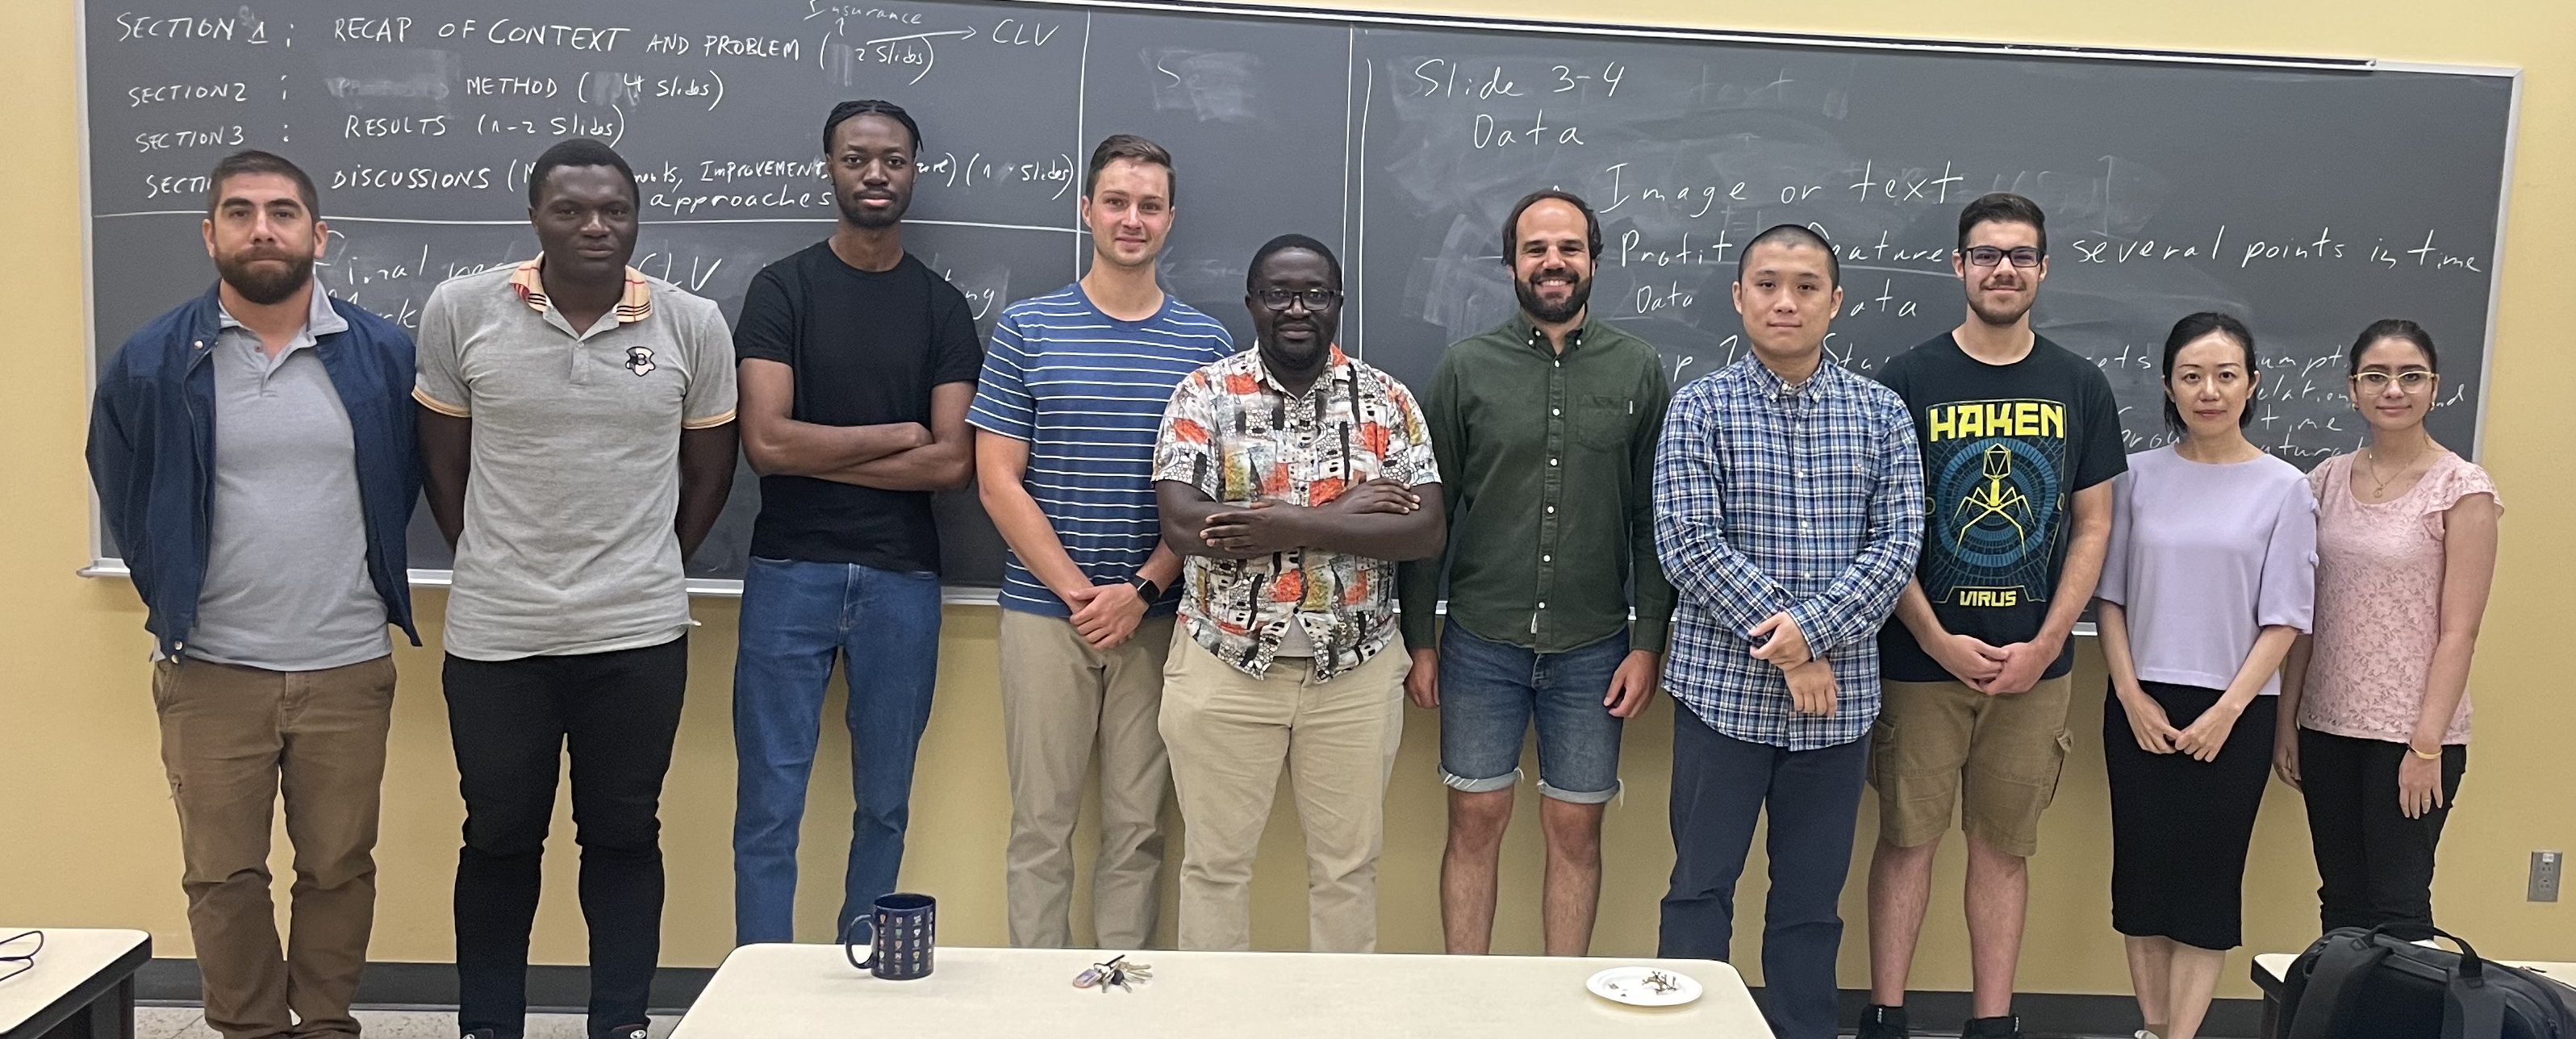
\includegraphics[width=10cm]{title_image.jpeg}}
%\institute{$13^e$ atelier de résolution de problèmes industriels de Montréal}
\date{August 25, 2023}

%%%%%%%%%%%%%%%%%%%%%%%%%%%%%%%%%%%%%%%%%%%%%%%%%%%%%%%%%%%%%%
%%%%%%%%%%%%%%%%%%%%%%%%%%%%%%%%%%%%%%%%%%%%%%%%%%%%%%%%%%%%%%

\begin{document}

\maketitle


\section{Introduction}

\begin{frame}
\frametitle{Insurance context}

\begin{itemize}
  \item \textbf{Providing Insights in a Complex Industry:}
  \begin{itemize}
    \item Insurance operations involve numerous variables, from risk assessment to customer behavior.
    \item \textbf{Customer Lifetime Value} (or CLV) offers a comprehensive metric encompassing these factors.
  \end{itemize}
  
  \item \textbf{Efficient Decision-Making:}
  \begin{itemize}
    \item CLV consolidates diverse information, streamlining decision processes.
    \item Enables optimized resource allocation, customer engagement, and tailored product offerings.
  \end{itemize}
\end{itemize}

\end{frame}

\begin{frame}
\frametitle{Customer Life Value (CLV)}

\begin{itemize}
    \item CLV represents the total expected profit a
    company expects from a client throughout their entire relationship.
    \item Used in multiple industries in order to evaluate the financial value of a
    customer and better tailor the approach of the company towards
    customers (pricing, marketing, etc.) 

\item Mathematically, we can define CLV as
\[
CLV(a) = \E\left[\sum_{t=1}^T \gamma^t Profit(S_t)\mid S_0 = a\right]
\]
where:
\begin{itemize}
    \item $\gamma$ is a discounting factor to account for time-value of money;
    \item $Profit(S_t)$ is a function that gives the expected profit from a client given their state $S_t$.
\end{itemize}

\end{itemize}
\end{frame}

\section{Method}

\begin{frame}
\frametitle{The model}

\begin{itemize}
	\item Problem: how to model $S_t$?
	\item Natural to think of $\{S_t\}$ as a sequence of r.v.
	\item We assume the Markov property for simplification:
\end{itemize}
\[ \Prob(S_{t+1} = s \mid S_t, S_{t-1}, \dots, S_0) = \Prob(S_{t+1} = s \mid S_t) \]
\\~\\
We used a method from Haenlein et al. (2007) that involves 3 steps:

\begin{enumerate}
	\item Fit a regression tree on the data to identify groups (i.e. the states of the Markov chain) with the profit as a target variable;
	\item Estimate the transition probabilities between each group/state;
	\item Compute the CLV by Monte Carlo.
\end{enumerate}

\end{frame}


\begin{frame}
\frametitle{Details}

\begin{figure}
	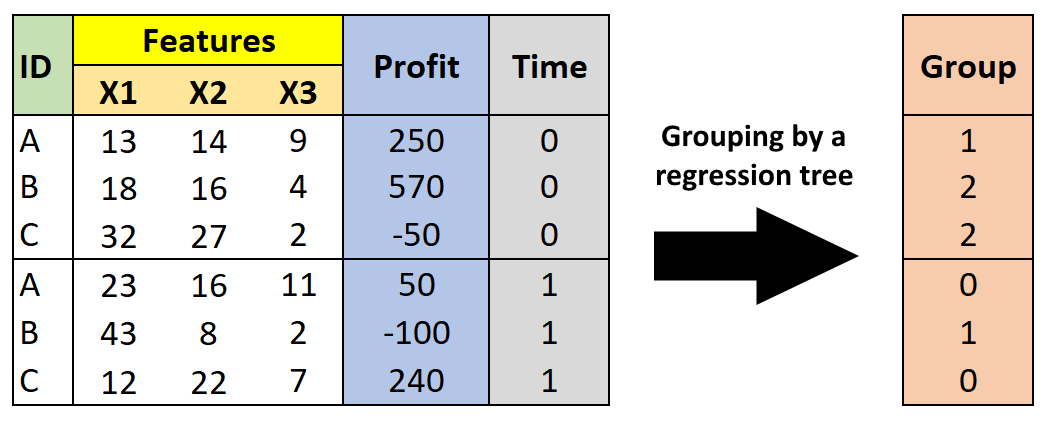
\includegraphics[scale = 0.3]{tree_result.jpg}
\end{figure}
	
\begin{itemize}
	\item \textbf{Step 1}: Combine data from all time steps into a single dataset (we assume time independency) and fit a regression tree;
	\item Result : that creates a new feature \textbf{Group} (there is a sense of order by profit). We can "forget" the other features from now on. 
\end{itemize}
\end{frame}

\begin{frame}
\frametitle{Details (continued)}

\begin{figure}
	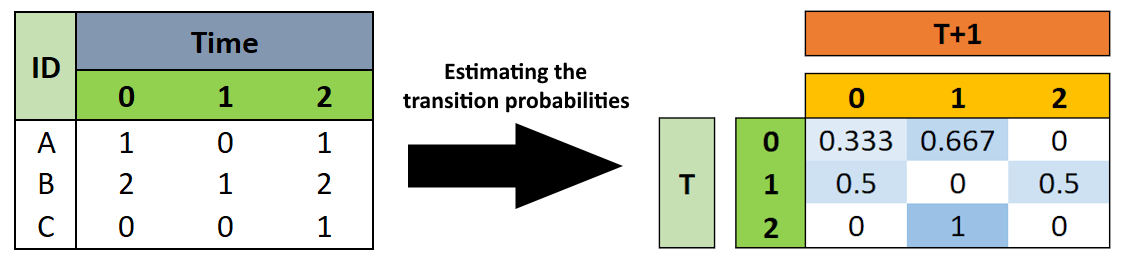
\includegraphics[scale = 0.4]{transitions.jpg}
\end{figure}
	
\begin{itemize}
	\item \textbf{Step 2}: Build the transition matrix with empirical transition probabilities (assuming time homogeneity);
	\item \textbf{Step 3}: Compute the CLV by simulating Markov chains (Monte Carlo method).
\end{itemize}
\end{frame}

\section{Discussion}

\begin{frame}
\frametitle{Other approaches}

\textbf{Extended Pareto/NBD Model}

\begin{itemize}
  \item Combines \textbf{Pareto/NBD} and \textbf{Gamma-Gamma} models.
  
  \item \textbf{Pareto/NBD Model}:
  \begin{itemize}
    \item Uses two main components: Pareto and Negative Binomial Distribution.
    \item Estimates parameters that describe customer behavior, such as transaction rate and the expected number of future transactions.
  \end{itemize}
  
  \item \textbf{Gamma-Gamma Model}:
  \begin{itemize}
    \item Assumes that customer transaction values follow a gamma distribution.
    \item Estimates parameters for average and variability in transaction values.
  \end{itemize}
  
  \item Gives \textbf{CLV predictions} by multiplying results from both submodels.
  
  \item Challenges Faced:
  \begin{itemize}
    \item Attempted implementation, but faced technical hurdles.
    \item The dataset provided for the workshop was not suited for implementation (missing variables).
  \end{itemize}
\end{itemize}

\end{frame}

\begin{frame}
\frametitle{References}

\begin{itemize}
	\item Haenlein, Michael \& Kaplan, Andreas \& Beeser, Anemone. (2007). \textit{A Model to Determine Customer Lifetime Value in a Retail Banking Context}. European Management Journal. 25. 221-234. 10.1016/j.emj 2007.01.004. 
\end{itemize}

\end{frame}

\end{document}
